\documentclass[10pt,aspectratio=169]{beamer} %Widescreen

\makeatletter
    \def\beamer@calltheme#1#2#3{%
        \def\beamer@themelist{#2}
        \@for\beamer@themename:=\beamer@themelist\do
        {\usepackage[{#1}]{\beamer@themelocation/#3\beamer@themename}}
    }

\def\usefolder#1{
    \def\beamer@themelocation{#1}
}
\def\beamer@themelocation{}

 
\usefolder{LRCgraphics}
\usetheme{LRC}
  
  
  
\definecolor{LRCcolorblue}{RGB}{24,77,127}
\definecolor{LRCcolorgrey}{RGB}{193,193,193}
% If you want to change the colors of the various elements in the theme, edit and uncomment the following lines

% Change the bar colors:
\setbeamercolor{LRC}{fg=LRCcolorgrey,bg=LRCcolorblue}
%\setbeamercolor{LRC}{fg=black!20,bg=black}

% Change the block colors:

\setbeamercolor{block title}{bg=LRCcolorblue,fg=white}

% Change the color of the structural elements:
\setbeamercolor{structure}{fg=black}

% Change the frame title text color:
%\setbeamercolor{frametitle}{fg=blue}

% Change the normal text color background:
\setbeamercolor{normal text}{fg=black,bg=gray!10}

% Change the Agenda:
\setbeamertemplate{section in toc}{%
  {\color{LRCcolorblue}\inserttocsectionnumber.}~\inserttocsection}
\setbeamercolor{subsection in toc}{bg=white,fg=structure}
\setbeamertemplate{subsection in toc}{%
  \hspace{1.2em}{\color{LRCcolorblue}\rule[0.3ex]{3pt}{3pt}}~\inserttocsubsection\par}


%Change color Itemize and Enumerate
  
\mode<presentation>
{
	\setbeamertemplate{enumerate items}[circle]
	\setbeamertemplate{itemize item}[square]
	\setbeamertemplate{itemize subitem}[circle]
	\setbeamertemplate{itemize subsubitem}[triangle]
	\setbeamercolor{item projected}{bg=LRCcolorblue}
    \setbeamercolor{itemize item}{fg=LRCcolorblue}
	\setbeamercolor{itemize subitem}{fg=LRCcolorblue}
	\setbeamercolor{itemize subsubitem}{fg=LRCcolorblue}
   
} 
%To achieve numbering of figures, you need to set: 
%\setbeamertemplate{caption}[numbered] 
 
%-------------------------------------------------------
% INCLUDE PACKAGES
%-------------------------------------------------------

\usepackage[utf8]{inputenc}
\usepackage[portuguese]{babel}
\usepackage[T1]{fontenc}
\usepackage{helvet}

%-------------------------------------------------------
% DEFFINING AND REDEFINING COMMANDS
%-------------------------------------------------------

% colored hyperlinks
\newcommand{\chref}[2]{
  \href{#1}{{\usebeamercolor[bg]{\theme\LRC}#2}}
}

%-------------------------------------------------------
% INFORMATION IN THE TITLE PAGE
%-------------------------------------------------------

\title[MC655 - LTE e Redes 5G]
{
    \textcolor{LRCcolorblue}{\textbf{Distribuição de Vídeo Multinível para Cidades Inteligentes}}
}

\subtitle[~]
{
    \vspace{0.3cm}
    \Small{\textbf{Exame de Qualificação Especifico}}
    \\ \vspace{0.3cm}
    \footnotesize{\textbf{Eduardo S. Gama}}
}

\author[Gama 2019]
{
    \footnotesize{
        \begin{tabular}{rl}
            \textbf{Orientador}:    & Luiz F. Bittencourt \\
            \textbf{Co-orientador}: & Roger Immich \\
        \end{tabular}
        % \textbf{Orientador:}    & \underline{Luiz F. Bittencourt} \\
        % \textbf{Co-orientador:} & \underline{Roger Immich}    \\
    }
}   

\institute[]
{
    Universidade Estadual de Campinas\\
    Instituto de Computação\\
    Laboratório de Redes de Computadores\\
}

\date{Campinas, \today}

%-------------------------------------------------------
% THE BODY OF THE PRESENTATION
%-------------------------------------------------------

\begin{document}

%-------------------------------------------------------
% THE TITLEPAGE
%-------------------------------------------------------

{\1
\begin{frame}[plain,noframenumbering]
\titlepage 
\end{frame}
}

%AGENDA
\begin{frame}{Agenda}{}
\tableofcontents
\end{frame}

%https://tecnoblog.net/218086/volte-ligacao-4g-ativar/

%Aparece menu a cada nova seção
\AtBeginSection[]
{
     \begin{frame}<beamer>
     \frametitle{Agenda}
     \tableofcontents[currentsection]
     \end{frame}
}

%-------------------------------------------------------
%INICIO
%-------------------------------------------------------
\section{Introdução}

%-=-=-=-=-=-=-=-=-=-=-=-=-=-=-=-=-=-=-=-=-=-=-=-=
%	FRAME: Introducao
%-=-=-=-=-=-=-=-=-=-=-=-=-=-=-=-=-=-=-=-=-=-=-=-=
\subsection{Increasing mobile data traffic}

\begin{frame}{Introdução}{Increasing mobile data traffic}
    \begin{itemize}
        \item Mobile data traffic is growing at a compound annual rate of 47%.
        \item In 2021 there will be 11,6 billion mobile-connected devices, exceeding the world’s projected population at that time (7,8 billion).
        \item Decisive factors:
        \begin{itemize}
            \item The popularity of internet applications
            \item The evolution of IoT devices.
        \end{itemize}
        % \item \textbf{3G}: Sistemas celulares com serviços de dados por pacotes e taxas maiores que 256 kbps.
        % \item \textbf{4G}: Sistemas projetados para oferecer taxas de download de 100Mbps com o usuário em movimento e 1Gbps com usuário parado. O uplink é de até 500Mbps.
        % \item \textbf{5G}: Novas aplicações.
    \end{itemize}
\begin{figure}[!htb]
    \centering
    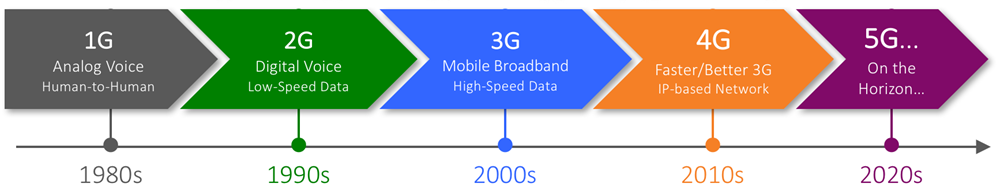
\includegraphics[scale=0.7]{LRCgraphics/5G-Evolution-Chart.png}
    \caption{Predicted video traffic growth by geography (2016–2021)~\cite{ciena5g2018}}
\end{figure}
\end{frame}
%-=-=-=-=-=-=-=-=-=-=-=-=-=-=-=-=-=-=-=-=-=-=-=-=
%	FRAME: 
%-=-=-=-=-=-=-=-=-=-=-=-=-=-=-=-=-=-=-=-=-=-=-=-=
\subsection{Evolução das tecnologias GSM -> 5G}
\begin{frame}{Introdução}{Evolução}

\begin{figure}[!htb]
    \centering
    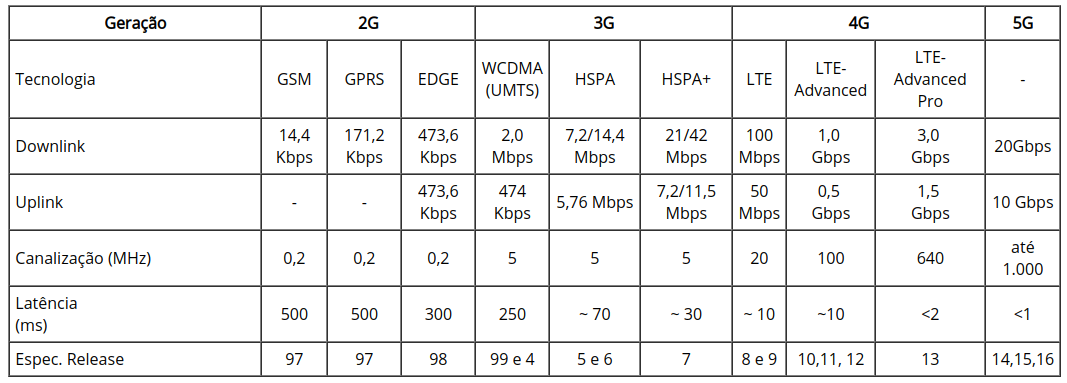
\includegraphics[scale=0.37]{LRCgraphics/evolucao_teleco.png}
    \caption{Evolução das tecnologias GSM \footnote{Mais informações: \url{http://www.teleco.com.br/tecnocel.asp}}}
\end{figure}

\end{frame}

\begin{frame}{Benefits of implementing Fog}
    \begin{itemize}
        \item Pre-processing,
        \item Geo-distribution,
        \item Low latency,
        \item Location/content awareness,
        \item Development and implementation of applications that involve:
        \begin{itemize}
            \item Complex data,
            \item Real-time interactions,
            \item Intensive processing.
        \end{itemize}
    \end{itemize}
\end{frame}

\begin{frame}{Taxa de dados média poara usuários}
\begin{figure}[!htb]
    \centering
    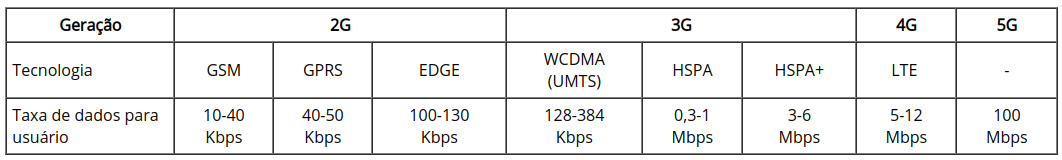
\includegraphics[scale=0.38]{LRCgraphics/taxadados_teleco.png}
    \caption{Downlink oferecido aos usuários pelas principais operadoras de banda larga móvel no Mundo}
\end{figure}
\end{frame}

% \begin{frame}{Tecnologias}
% \begin{itemize}
%     \item AMPS $\rightarrow$ FDMA
%     \item GSM $\rightarrow$ FDMA + TDMA
%     \item GPRS
%     \item EDGE
%     \item WCDMA (UMTS)
%     \item HSPA
%     \item HSPA+
%     \item LTE
% \end{itemize}
% \end{frame}

\begin{frame}{Evolução das tecnologias de celular no Brasil}
\begin{figure}[!htb]
    \centering
    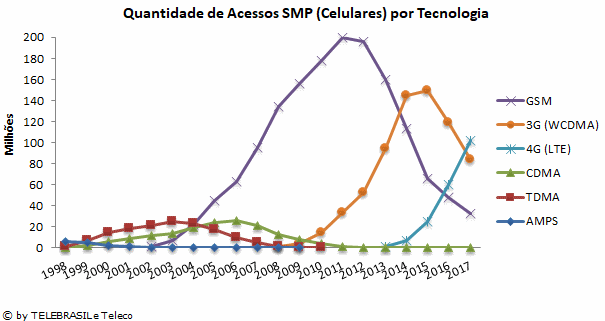
\includegraphics[scale=0.45]{LRCgraphics/tecnocel2017_teleco.png}
    \caption{Uso das tecnologias celulares no Brasil de 1998 a 2017\footnote{Mais informações: \url{http://www.teleco.com.br/ncel.asp}}}
\end{figure}
\end{frame}
%-=-=-=-=-=-=-=-=-=-=-=-=-=-=-=-=-=-=-=-=-=-=-=-=
%	FRAME: 
%-=-=-=-=-=-=-=-=-=-=-=-=-=-=-=-=-=-=-=-=-=-=-=-=
\section{LTE}
\begin{frame}{LTE}
\flushleft
    \begin{itemize}
        \item O LTE (\textbf{L}ong \textbf{T}erm \textbf{E}volution) é o termo adotado para designar o padrão de 4ª Geração estabelecido para a rede das operadoras de celular como evolução para operadoras de GSM.
        \item Especificações são publicadas pelo 3GPP (3rd Generation Partnership Project).
        \item Releases: 8 e 9 (LTE); 10, 11 e 12 (LTE-A); e 13 (LTE-A Pro)
    \end{itemize}
% \begin{figure}[!htb]
%     \centering
%     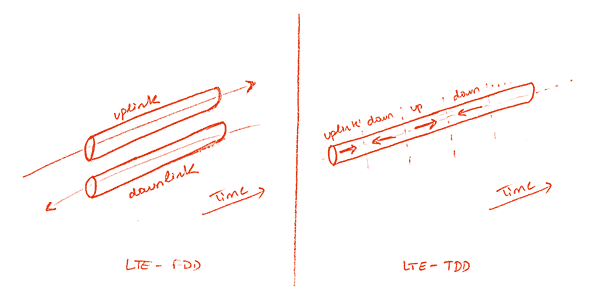
\includegraphics[scale=0.38]{LRCgraphics/LTE-FDD-TDD.png}
%     \caption{Funcionamento do FDD e TDD no LTE}
% \end{figure}
\end{frame}
%-=-=-=-=-=-=-=-=-=-=-=-=-=-=-=-=-=-=-=-=-=-=-=-=
%	FRAME: 
%-=-=-=-=-=-=-=-=-=-=-=-=-=-=-=-=-=-=-=-=-=-=-=-=
\begin{frame}{LTE cont.}
    \begin{itemize}
        \item Utilização de modos FDD (\textit{Frequency Division Duplex}) e TDD (\textit{Time Division Duplex}) para os Users Equipments (UEs) se comunicarem com as estações base (eNodeB).
    \end{itemize}
\begin{figure}[!htb]
    \centering
    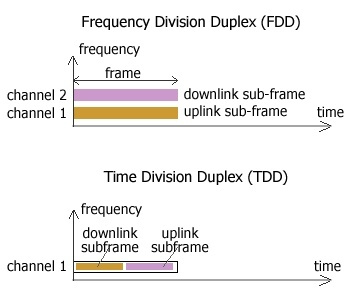
\includegraphics[scale=0.45]{LRCgraphics/fdd_tdd-2.jpg}
    \caption{Funcionamento do FDD e TDD no LTE \cite{carvalho2013}}
\end{figure}
\end{frame}
%-=-=-=-=-=-=-=-=-=-=-=-=-=-=-=-=-=-=-=-=-=-=-=-=
%	FRAME: 
%-=-=-=-=-=-=-=-=-=-=-=-=-=-=-=-=-=-=-=-=-=-=-=-=
\subsection{Características}
\begin{frame}{LTE}{Características}
    \begin{itemize}
        \item Altas taxas de dados
        \begin{itemize}
            \item Download: 100 Mbps
            \item Upload: 50 Mbps
        \end{itemize}
        \item Baixa latência: $\sim$10 ms
        \item Comunicação de voz por IP, denominado VoIP
        \item Flexibilidade de largura de rádio
        \item Núcleo de pacote desenvolvido (EPC -Evolved Packet Core) \cite{epc3gpp}
        \item Rede de acesso por rádio LTE
        \item OFDMA (Orthogonal Frequency Division Multiple Access)
        \item Tecnologia de antena MIMO (Multiple Input Multiple Output)
    \end{itemize}
\end{frame}

\begin{frame}{LTE}{Características}
\begin{table}[]
\begin{tabular}{l|l|l|l|l|l}
%\hline
Tecnologia      & Downlink\footnote{ERB $\rightarrow$ Celular} & Uplink\footnote{Celular $\rightarrow$ ERB}   & Canalização (MHz) & Latência (ms) & Release     \\ \hline
LTE             & 100 Mbps & 50 Mbps  & 20                & $\sim$~10      & 8 e 9       \\ \hline
LTE-A           & 1.0 Gbps & 0.5 Gbps & 100               & $\sim$~10      & 10, 11 e 12 \\ \hline
LTE-A Pro       & 3.0 Gbps & 1.5 Gbps & 640               & $\textless$~2   & 13         \\
%\hline
\end{tabular}
\caption{Principais características das redes LTE}
\end{table}

\end{frame}
%-=-=-=-=-=-=-=-=-=-=-=-=-=-=-=-=-=-=-=-=-=-=-=-=
%	FRAME: 
%-=-=-=-=-=-=-=-=-=-=-=-=-=-=-=-=-=-=-=-=-=-=-=-=
\subsection{Arquitetura}
\begin{frame}{LTE}{Arquitetura}
\begin{figure}[!htb]
    \centering
    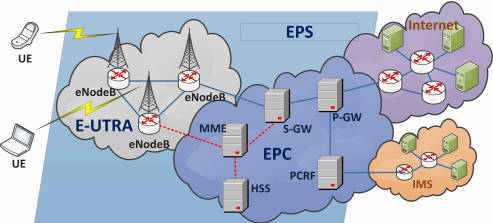
\includegraphics[scale=0.7]{LRCgraphics/The-LTE-Architecture.png}
    \caption{Arquitetura do LTE \cite{liyanage2015leveraging}}
    % 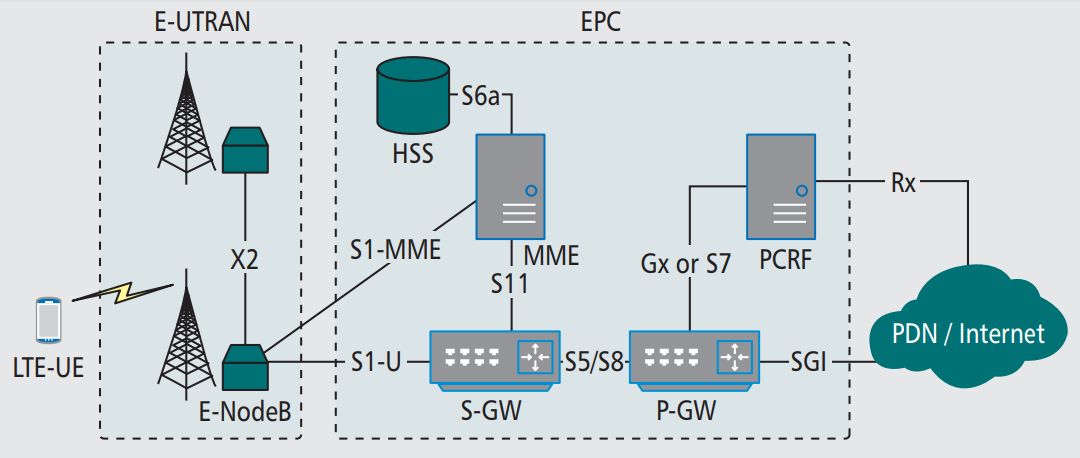
\includegraphics[scale=0.34]{LRCgraphics/lte_arc.png}
    % \caption{Arquitetura do LTE \cite{bradai2015cellular}}
\end{figure}
\end{frame}
%-=-=-=-=-=-=-=-=-=-=-=-=-=-=-=-=-=-=-=-=-=-=-=-=
%	FRAME: 
%-=-=-=-=-=-=-=-=-=-=-=-=-=-=-=-=-=-=-=-=-=-=-=-=
\begin{frame}{LTE}{Arquitetura - EPC (Evolved Packet Core)}
    \begin{itemize}
        \item MME (Mobility Management Entity):
        \item S-GW (Serving Gateway):
        \item P-GW(Packet Data Network Gateway):
        \item PCRF (Policy and Charging Rules Function):
        \item HSS (Home Subscriber Server):
    \end{itemize}
\end{frame}
%-=-=-=-=-=-=-=-=-=-=-=-=-=-=-=-=-=-=-=-=-=-=-=-=
%	FRAME: 
%-=-=-=-=-=-=-=-=-=-=-=-=-=-=-=-=-=-=-=-=-=-=-=-=
\begin{frame}{LTE}{Arquitetura - E-UTRAN (Evolded Universal Terrestrial Radio Access Network)}
    \begin{itemize}
        \item UE (User Equipment):
        \item Interface X2: %\url{http://www.teleco.com.br/tutoriais/tutorialltemcp/pagina_4.asp}
        \item eNodeB (Evolved Node B):
    \end{itemize}
\end{frame}
%-=-=-=-=-=-=-=-=-=-=-=-=-=-=-=-=-=-=-=-=-=-=-=-=
%	FRAME: 
%-=-=-=-=-=-=-=-=-=-=-=-=-=-=-=-=-=-=-=-=-=-=-=-=
\begin{frame}{LTE}{Arquitetura - Estrutura do Frame}
    \begin{itemize}
        \item UE (User Equipment):
        \item Interface X2: %\url{http://www.teleco.com.br/tutoriais/tutorialltemcp/pagina_4.asp}
        \item eNodeB (Evolved Node B):
    \end{itemize}
\end{frame}
%-=-=-=-=-=-=-=-=-=-=-=-=-=-=-=-=-=-=-=-=-=-=-=-=
%	FRAME: 
%-=-=-=-=-=-=-=-=-=-=-=-=-=-=-=-=-=-=-=-=-=-=-=-=
\subsection{Modulação}
\begin{frame}{LTE}{OFDMA}
\begin{figure}[!htb]
    \centering
    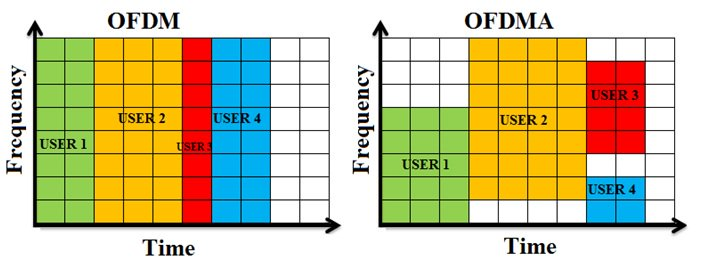
\includegraphics[scale=0.6]{LRCgraphics/difference-between-ofdm-and-ofdma.jpg}
    \caption{OFDM e OFDMA}
\end{figure}
\end{frame}
%-=-=-=-=-=-=-=-=-=-=-=-=-=-=-=-=-=-=-=-=-=-=-=-=
%	FRAME: 
%-=-=-=-=-=-=-=-=-=-=-=-=-=-=-=-=-=-=-=-=-=-=-=-=
\subsection{Modulação}
\begin{frame}{LTE}{MIMO}
\begin{figure}[!htb]
    \centering
    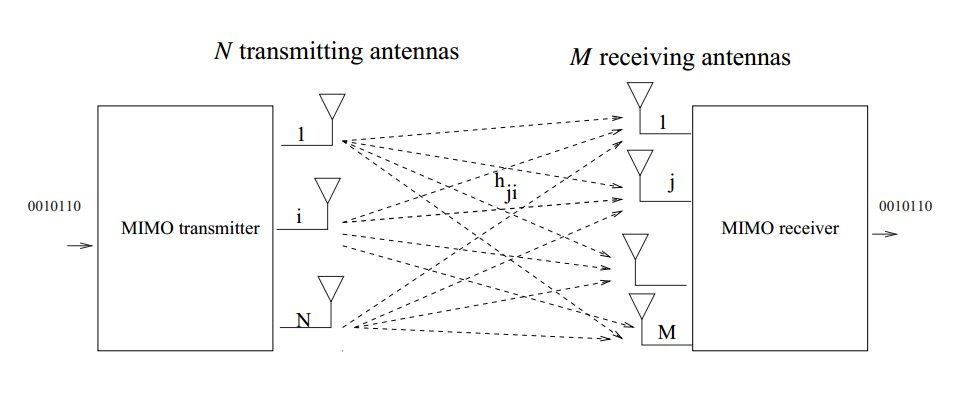
\includegraphics[scale=0.5]{LRCgraphics/mimo.png}
    \caption{MIMO LTE \cite{mimogta2014}}
\end{figure}
\end{frame}
%-=-=-=-=-=-=-=-=-=-=-=-=-=-=-=-=-=-=-=-=-=-=-=-=
%	FRAME: 
%-=-=-=-=-=-=-=-=-=-=-=-=-=-=-=-=-=-=-=-=-=-=-=-=
\subsection{Qualidade de Serviço e Experiência}
\begin{frame}{LTE}{Qualidade de Serviço e Experiência}
    \begin{itemize}
        \item teste 1
    \end{itemize}
\end{frame}
%-=-=-=-=-=-=-=-=-=-=-=-=-=-=-=-=-=-=-=-=-=-=-=-=
%	FRAME: 
%-=-=-=-=-=-=-=-=-=-=-=-=-=-=-=-=-=-=-=-=-=-=-=-=
\subsection{LTE-Advanced e LTE-Advanced Pro}
\begin{frame}{LTE-A e LTE-A Pro}
\begin{itemize}
    \item LTE-A: o dispositivo celular se conecta a mais de uma frequência ou faixa de espectro.
    \item LTE-A Pro: O LTE-A em suas melhores condições.
    \begin{itemize}
        \item Agregação de portadora: combinar três diferentes faixas de frequência.
        \item MIMO 4x4: 4 antenas para transmissão e 4 para recepção;
        \item Modulação 256QAM: maior eficiência espectral, transmitindo mais bits de dados a cada tempo. Mais dados simultaneamente.
    \end{itemize}
\end{itemize}
\begin{figure}[!htb]
    \centering
    
\includegraphics[scale=0.3]{LRCgraphics/LTE_logos.png}
    \caption{Evoluções do LTE ao longo dos anos}
\end{figure}
\end{frame}
%-=-=-=-=-=-=-=-=-=-=-=-=-=-=-=-=-=-=-=-=-=-=-=-=
%	FRAME: 
%-=-=-=-=-=-=-=-=-=-=-=-=-=-=-=-=-=-=-=-=-=-=-=-=
\section{VoLTE}
\begin{frame}{VoLTE}
    \begin{itemize}
        \item teste 1
    \end{itemize}
\end{frame}

%-=-=-=-=-=-=-=-=-=-=-=-=-=-=-=-=-=-=-=-=-=-=-=-=
%	FRAME: 5G
%-=-=-=-=-=-=-=-=-=-=-=-=-=-=-=-=-=-=-=-=-=-=-=-=
\section{Redes 5G}
\begin{frame}{Redes 5G}
    \centering
    \Large{\textbf{Redes 5G...}}
\end{frame}
%-=-=-=-=-=-=-=-=-=-=-=-=-=-=-=-=-=-=-=-=-=-=-=-=
%	FRAME: Referencias
%-=-=-=-=-=-=-=-=-=-=-=-=-=-=-=-=-=-=-=-=-=-=-=-=
\begin{frame}[allowframebreaks]{Referências}
\small{
    \bibliography{referencias}
}
\bibliographystyle{IEEEtran}
\end{frame}


%-------------------------------------------------------
%FINAL
%-------------------------------------------------------
{\1
\begin{frame}[plain,noframenumbering]
  \finalpage{\large{
  \textbf{Obrigado!} \\
  \vspace{0.2cm}
  \url{www.lrc.ic.unicamp.br/~joahannes} \\
  \url{www.lrc.ic.unicamp.br/~wellington}
  }}
\end{frame}
}

\end{document}